\section{Superpixel propagation for object segmentation in videos}
\label{sec:segm}
The algorithm proposed in \cite{c18}, offers a good deal in terms of
background-foreground separation from user interaction. A technique like this, however,
performs very well in still images, but it may not be well adapted for sequential videos, 
Extensions to this method, like GrabCut (\cite{c14}), work by implementing an iterative graph cut based 
minimization to separate regions according to appearance information, that can be
extracted from the user interaction. This interaction, however, could be minimized in videos,
given the extra information that offers the flow of the sequence.
Some authors had approached the GrabCut or similar graph based segmentation techniques in sequential
videos, to propagate a consistent segmentation \cite{c15}.
However, some more work on reducing user interaction given the extra flow-like information
that video sequences offer is still needed.
We propose to combine the presented superpixel flow as an automatic method to initialize the
desired min-cut max flow based algorithm to perform object
segmentation through frames in a video sequence. \\

The main idea consist in tracking (or more exactly, match) superpixels that are labeled as background, 
thanks to an object tracker initialization. Thus, the superpixels that are initially outside the ROI, 
can be propagated through the sequence, and if they fall into the ROI of the next frame, they
can be safely labeled as background again. We call this process background segments tarcking. 
The process is repeated for any labeled superpixel through the video. Having several labeled superpixels can 
reduce widely or totally the necessity for user interaction in subsequent frames. Thus, to perform object segmentation in a full video sequence, the required
user interaction would only be the initial bounding box. Moreover, a fully automatic approach can be
obtained if a reliable object detector is available.

Fig. \ref{figurelabel_walking} shows the results for an image sequence where the interest object is the head of a person.
The head tracker and the superpixel flow provide information for better background-foreground separation. The
background-foreground models are updated as the frames go on, giving more robustness for sequential
propagation of the segmentation. The method is tested in the Walking Couple sequence, by allowing only a small amount of iterations in the
graph based segmentation. Observe how the contour in the man's head is correctly delineated when
another person's head occludes part of it. In this case, the superpixels that belong to the woman’s face
were correctly propagated and thus, labeled as background. \\
   \begin{figure}[thpb]
      \centering
      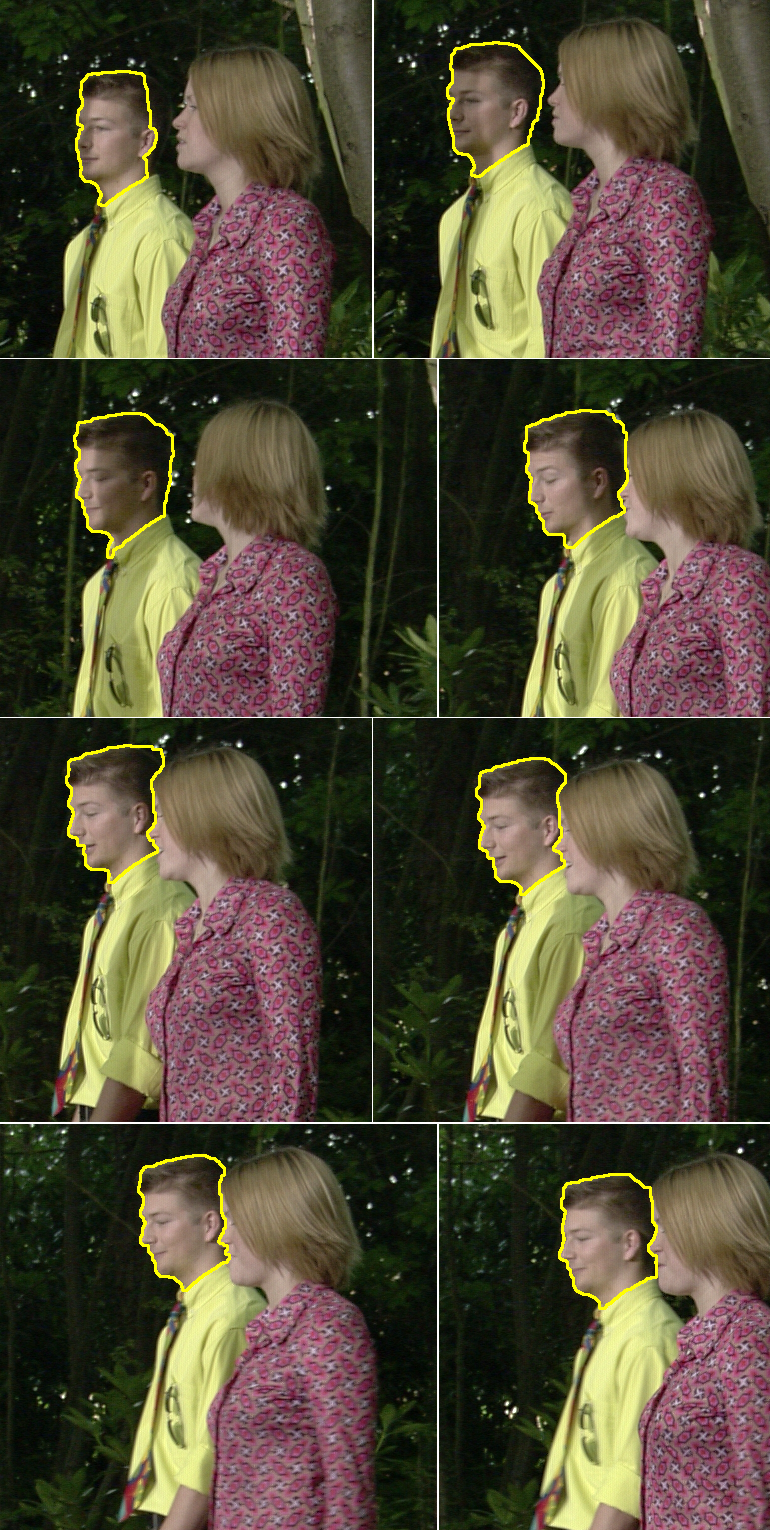
\includegraphics[height=0.75\textheight]{images/Sequence2.png}
      \caption{Segmentation through the sequence “Walking
	       Couple” (Yellow contour) initialized in the man’s head. The yellow box correspond to the tracker output.}
      \label{figurelabel_walking}
   \end{figure}

In order to understand the effect of including superpixel propagation in a video sequence for object
segmentation, some results are shown in the Fig. \ref{figurelabel_comp}. For these experiments only one iteration is
allowed in two grab-cut based methods. One initialized only with the tracker, and the other complemented with the superpixel
propagation. Observe that in general, the contour delineated is usually better in terms of precision and
stability for the later one.
   \begin{figure}[thpb]
      \centering
      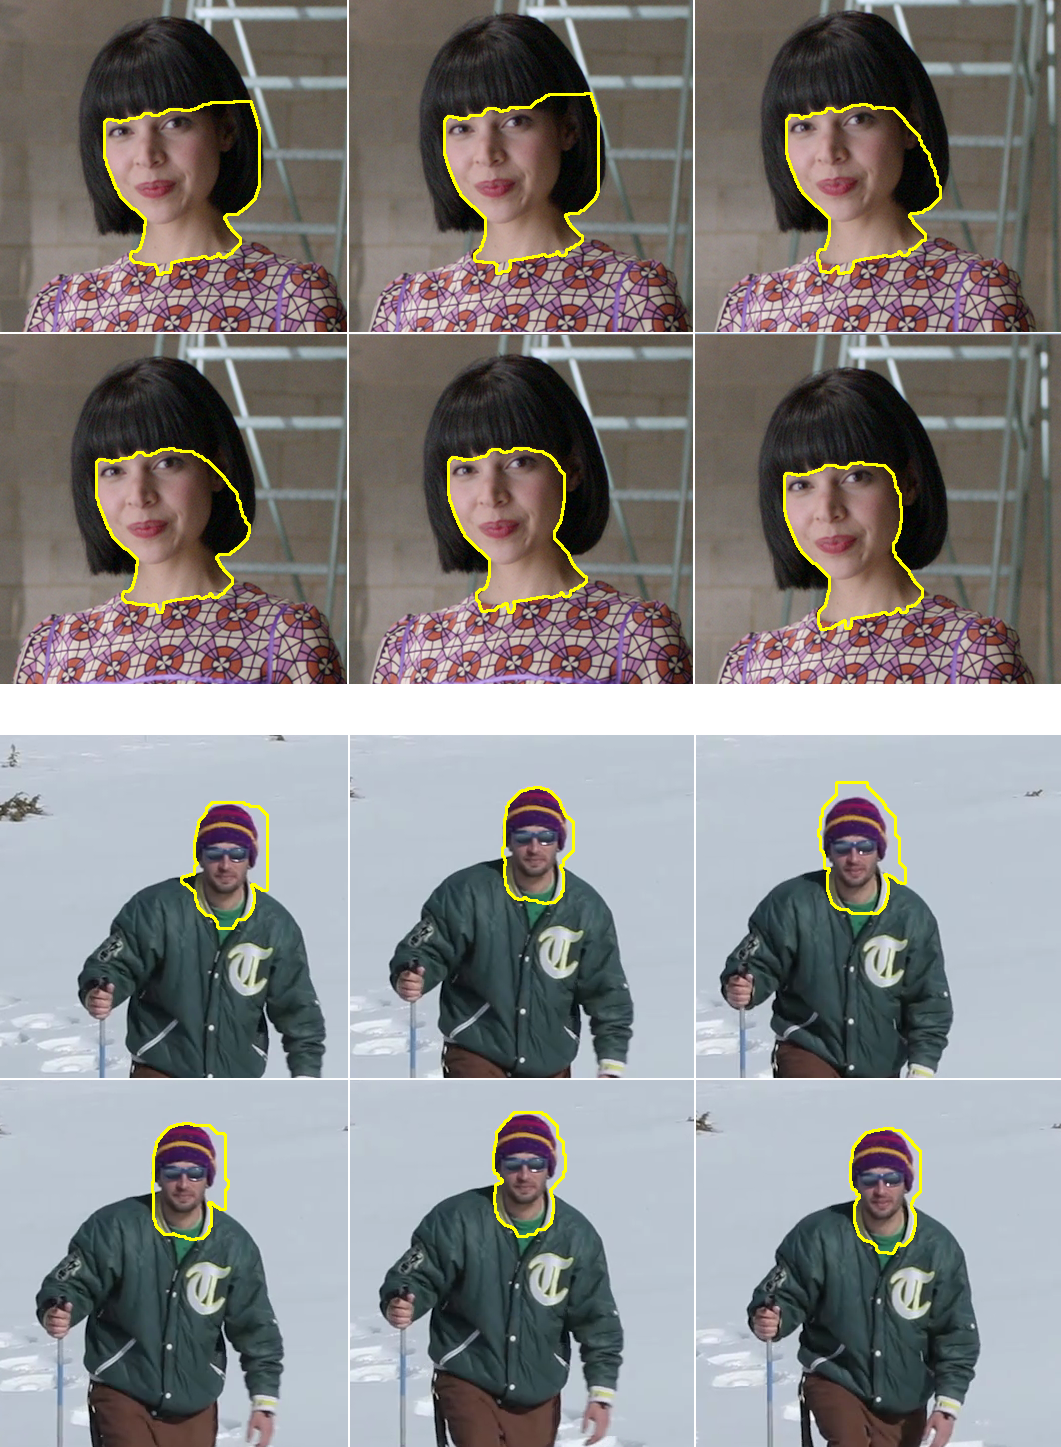
\includegraphics[height=0.66\textheight]{images/Compare.png}
      \caption{Face segmentation in the “Amelie Retro” and the
	      “Snow shoes” sequences in three different frames. For each
	       group, the Top Row: One-iteration window-based grabcut;
	       and the Bottom Row: One-iteration grabcut with super pixel
	       propagation.}
      \label{figurelabel_comp}
   \end{figure}